\chapter{Styling components}

\section{Video: StyleSheet API}
\begin{itemize}
  \item Extract styles from the component's render, keeping all the styles together.
  \item Inline styling is when you keep all the styles within the components render. As your application grows, this method of inline styling can get unmanageable very quickly and the code is harder to read. 
  \item React Native provides a style sheet which is an API that is very similear to CSS style sheets.
  \item StyleSheet API allow moving styles away from the components render.
  \item Using:
  \begin{lstlisting}[language=Java, numbers=none]
    <View style={styles.container}>
      <Text style={styles.title}>Hello World</Text>
    </View>

    const styles = StyleSheet.create({
      container: {
        ...
      },
      title: {
        ...
      }
    })
  \end{lstlisting}
  \item We can create a \texttt{global style} folder to reuse all the style for our components.
  \item \textbf{Practive Question:} The \texttt{StyleSheetAPI} helps abstract the component styles from the component's render and results inreadable and meaningful code.  True or false?
    $\rightarrow$ True
\end{itemize}

\section{Video: Practical Styling}
\begin{itemize}
  \item Convert previous work of MenuItems using StyleSheet:
  \begin{lstlisting}[language=Java, numbers=none]
    <View style={menuStyle.container}>
      <ScrollView
        style={menuStyle.innerContainer}>
        <Text style={menuStyle.headerText}>
          View Menu
        </Text>
        <Text style={menuStyle.itemText}>
          {menuItemsToDisplay[0]}
        </Text>
      </ScrollView>
    </View>

    const menuStyle = StyleSheet.create({
      container: {
        flex: 0.75
      },
      innerContainer: {
        paddingHorizontal: 40,
        paddingVertical: 40,
        backgroundColor: 'black',
      },
      headerText: {
        color: 'white',
        fontSize: 40,
        flexWrap: 'wrap'
      },
      itemText: {
        color: '#F4CE14',
        fontSize: 36
      }
    })
  \end{lstlisting}
  \item Convert Header style:
  \begin{lstlisting}[language=Java, numbers=none]
    import { View, Text, StyleSheet } from 'react-native';

    export default function LittleLemonHeader() {
      return (
        <View style={headerStyle.container}>
          <Text
            style={headerStyle.headerText}>
            Little Lemon
          </Text>
        </View>
      );
    }

    const headerStyle = StyleSheet.create({
      container: {
        backgroundColor: '#F4CE14'
      },
      headerText: {
        padding: 40,
        fontSize: 30,
        color: 'black',
        textAlign: 'center'
      }
    })
  \end{lstlisting}

  \item Convert App:
  \begin{lstlisting}[language=Java, numbers=none]
    import { StyleSheet, View } from 'react-native';
    import LittleLemonHeader from './components/LittleLemonHeader';
    import MenuItems from './components/MenuItems';
    export default function App() {
      return (
        <>
          <View
            style={style.container}
          >
            <LittleLemonHeader />
            <MenuItems />
          </View>
        </>
      );
    }

    const style = StyleSheet.create({
      container: {
        flex: 1,
        backgroundColor: '#495E57'
      }
    })
  \end{lstlisting}
\end{itemize}

\section{Reading: Styling using StyleSheet}
This section is to style all the components that I have done in the previous part.

\section{Reading: Exercise: Style a component}
\begin{itemize}
  \item This part follow the same above process.
  \item Header convert: 
  \begin{lstlisting}[language=Java, numbers=none]
    import { View, Text, StyleSheet } from 'react-native';

    export default function LittleLemonHeader() {
      return (
        <View style={headerStyle.container}>
          <Text
            style={headerStyle.headerTitle}
          >
            Little Lemon
          </Text>
        </View>
      );
    }

    const headerStyle = StyleSheet.create({
      container: {
        backgroundColor: '#F4CE14'
      },
      headerTitle: {
        padding: 40,
        fontSize: 30,
        color: 'black',
        textAlign: 'center'
      }
    })
  \end{lstlisting}
  \item Footer convert:
  \begin{lstlisting}[language=Java, numbers=none]
    import * as React from 'react';
    import { View, Text, StyleSheet } from 'react-native';

    export default function LittleLemonFooter() {
      return (
        <View
          style={footerStyle.container}
        >
          <Text
            style={footerStyle.footerTitle}
          >
            All rights reserved by Little Lemon, 2022{' '}
          </Text>
        </View>
      );
    }

    const footerStyle = StyleSheet.create({
      container: {
        backgroundColor: '#F4CE14',
        marginBottom: 10,
      },
      footerTitle: {
        fontSize: 18,
        color: 'black',
        textAlign: 'center',
      }
    }) 
  \end{lstlisting}
  \item Main app convert:
  \begin{lstlisting}[language=Java, numbers=none]
    import * as React from 'react';
    import { StyleSheet, View } from 'react-native';

    import LittleLemonHeader from './components/LittleLemonHeader';
    import LittleLemonFooter from './components/LittleLemonFooter';
    import WelcomeScreen from './WelcomeScreen';

    export default function App() {
      return (
        <>
          <View
            style={style.HeaderContainer}
          >
            <LittleLemonHeader />
            <WelcomeScreen />
          </View>
          <View 
            style={style.FooterContainer}
          >
            <LittleLemonFooter />
          </View>
        </>
      );
    }

    const style = StyleSheet.create({
      HeaderContainer: {
        flex: 1,
        backgroundColor: '#495E57',
      },
      FooterContainer: {
        backgroundColor: '#495E57'
      }
    })
  \end{lstlisting}
\end{itemize}

\section{Self review: Style a component}
\begin{figure}[H]
  \centering
  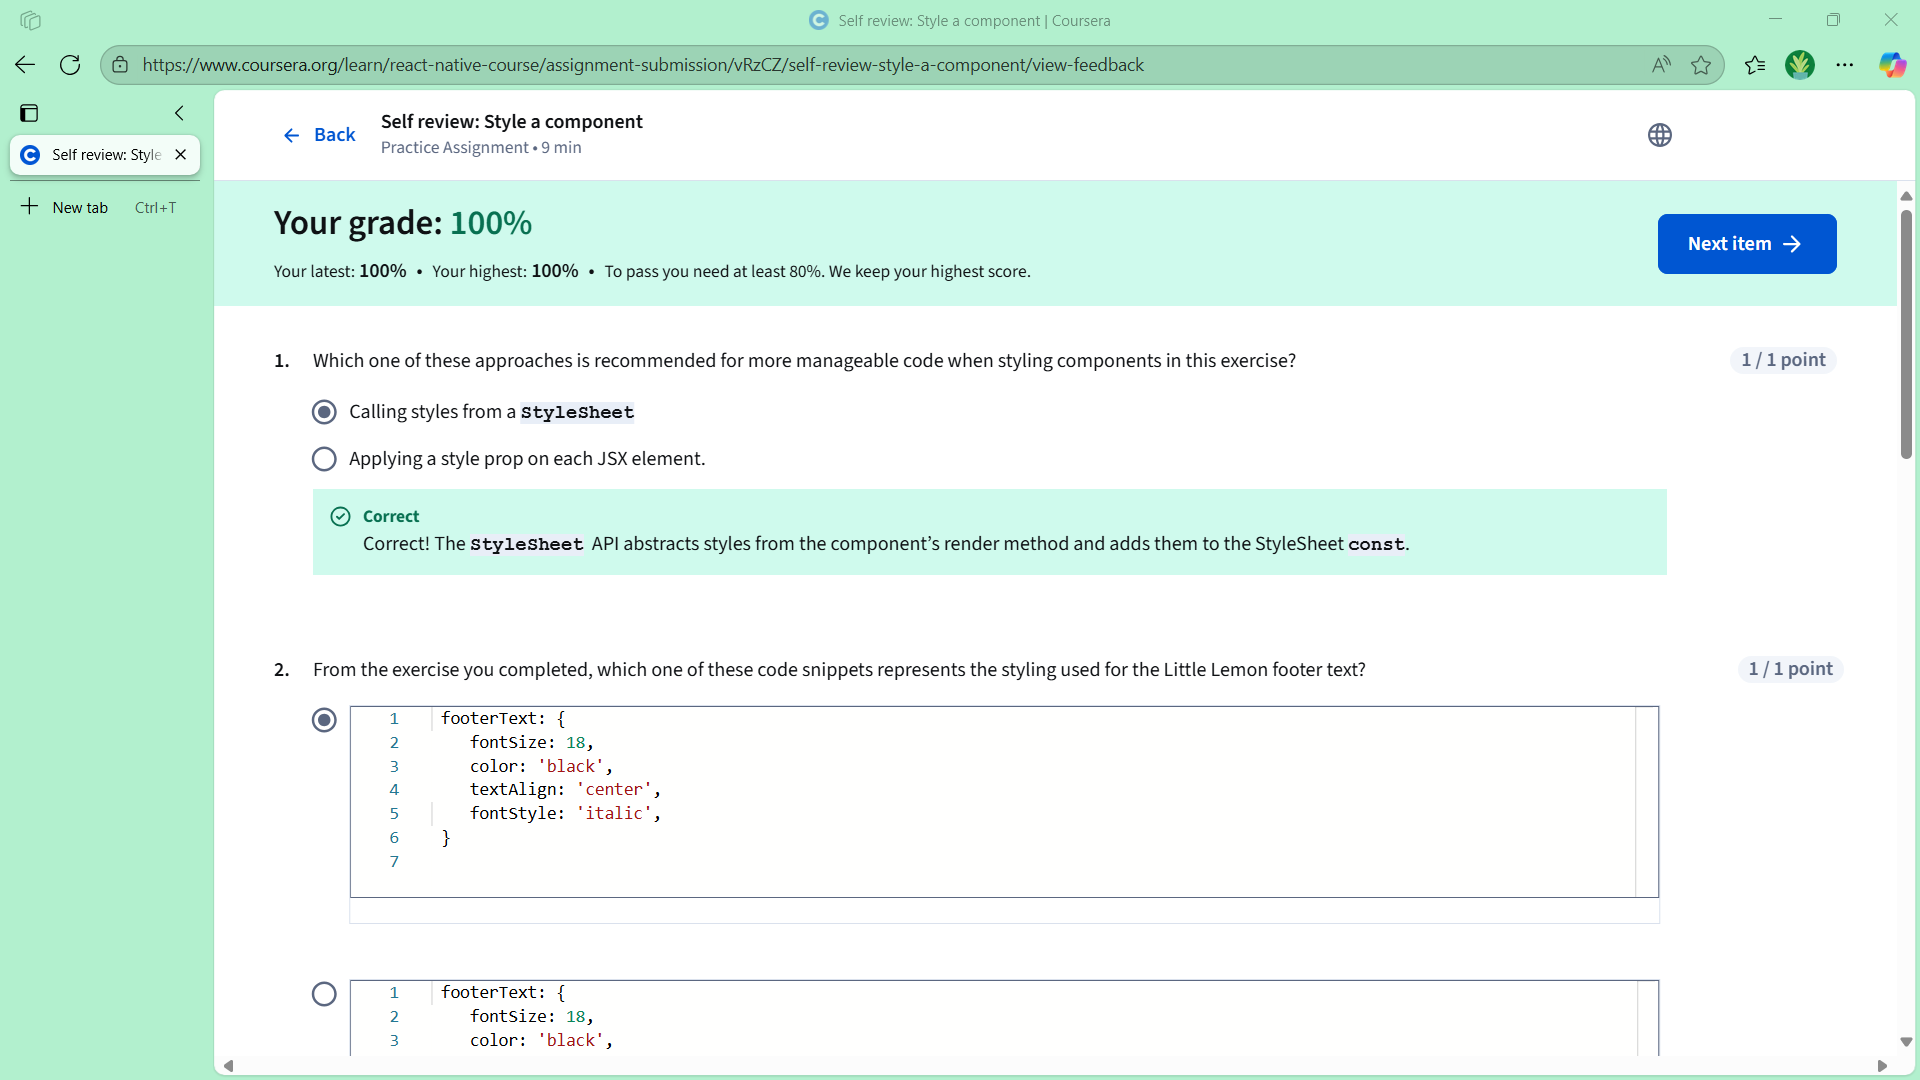
\includegraphics[width=0.5\linewidth]{images/self-review-4.png}
  \caption{Self review: Style a component}
\end{figure}

\section{Video: Module summary: Introduction to React Native}
\textbf{Introduction to React Native}
\begin{itemize}
  \item What is React Native
  \item Motivation behind using React Native
  \item Roles
\end{itemize}

\textbf{Introduction to React Native}
\begin{itemize}
  \item How to be successful
  \item Setup React Native Project
\end{itemize}

\textbf{Why React Native}
\begin{itemize}
  \item Describe the basics of React Native
  \item Benefits of React Native
  \item React Native in the real world
\end{itemize}

\textbf{React Native and Expo}
\begin{itemize}
  \item What is Expo
  \item How to build an app with Expo code
\end{itemize}

\textbf{Components}
\begin{itemize}
  \item Categorize React Native
  \item Use components to build apps
  \item Give an overview about React Native's components
\end{itemize}

\textbf{Views and Text}
\begin{itemize}
  \item Demonstate the use of View and Text
  \item Describe basic features of View and Text
\end{itemize}

\textbf{ScrollView}
\begin{itemize}
  \item Demonstate how to build a scrollable view
  \item Describe where you will use a scrollable view
\end{itemize}

\textbf(React Native Styling)
\begin{itemize}
  \item Inline styling
  \item Benefits of using stylesheets
  \item Practical Styling
\end{itemize}

\section{Module quiz: Introduction to React Native}
\begin{figure}[H]
  \centering
  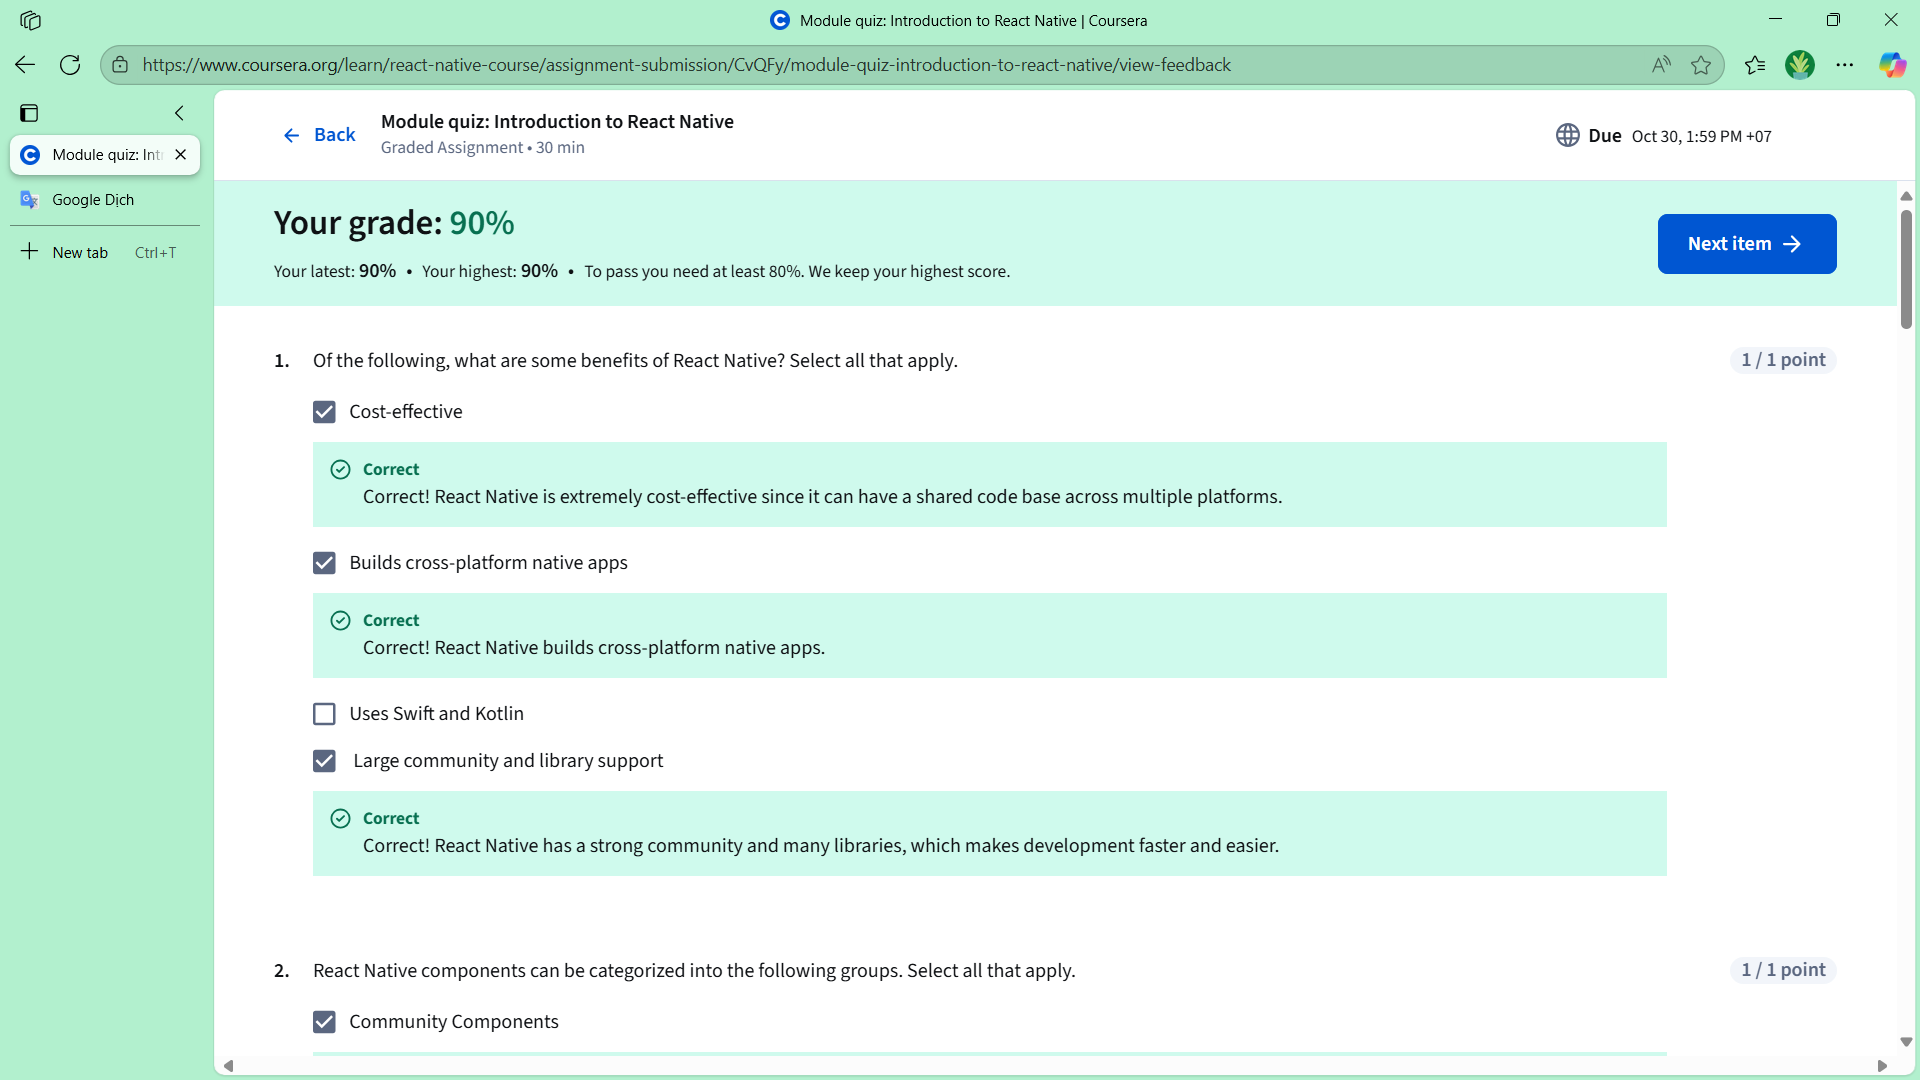
\includegraphics[width=0.5\linewidth]{images/module-quiz-1.png}
  \caption{Module quiz: Introduction to React Native}
\end{figure}